  \chapter{Lokale Flächentheorie im euklidischen Raum}
\section{Grundbegriffe der Flächentheorie}
\setcounter{subsection}{-1}
\subsection{$p$-dimensionale Flächen im affinen $\IR^n$}
Sei \(1 < p < n\) fest gewählt (in Anwendungen meist \(p = 2, n= 3\)).
 
\begin{definition}[Parametrisierte \(\C^r\)-\(p\)-Fläche (\(r \ge 0\))]\index{Fläche}
\(\C^r\)-Abbildung \(x\colon G \subset \IR^p \to \IR^n\)
\[
 u = \left( u^1, \dots , u^p \right) \mapsto x(u) = \left(x^1(u), \dots, x^n (u) \right) 
\]
wobei \(G\) ein \uline{Gebiet} des \(\IR^p\) (d.h. offen und zusammenhängend) ist.\\
\uline{Parameter:}\index{Fläche!Parameter} \[ u^1, \dots , u^p \quad \text{bei }n = 3\text{ meist }(u,v) \]
\uline{Parameterlinien:}\index{Fläche!Parameterlinie}
\[u^\varrho \mapsto x \left(u^1_0, \dots , u^\varrho , \dots , u^p_0 \right)\]
\uline{Spur:}\index{Fläche!Spur} \[M:= x\left[G \right] \subset \IR^n\]
\uline{Regularität \(r \geq 1\)}\index{Fläche!regulär}: Die partiellen Ableitungen 
\[x_\varrho := \partial_\varrho x = \frac{\partial x}{\partial u^\varrho} \quad (\varrho = 1, \dots , p)\] 
sind überall linear unabhängig (sonst \uline{Singularitäten})\index{Fläche!Singularität}.
\end{definition}

\begin{bemerkung}\(\)
\begin{enumerate}
 \item Regularität bedeutet: Die partiellen Ableitungen \(x_\varrho (\varrho = 1, \ldots , p)\) [\underline{"`Tangentialvektoren"'}] spannen überall einen p-dimensionalen \uline{Tangentialraum}\index{Tangentialraum} auf. Es gibt keine "`Grate"' oder schlimmeres.
 \item Reguläre parametrisierte \(p\)-Flächen sind \uline{lokal injektiv}; die Funktionalmatrix 
\[Dx = \left(\frac{\partial (x^1, \dots , x^n)}{\partial (u^1, \ldots , u^p)}\right) = \left(x_1, \ldots , x_p\right)\]
besitzt überall den Höchstrang \(p\) (Satz über implizite Funktionen). Bei lokalen Untersuchungen kann man stets annehmen, dass \(x \colon G \subset \IR^p \rightarrow x \left[G \right] = M \subset \IR^n\) bijektiv ist, also keine Selbstdurchdringungen auftreten. Eine parametrisierte \uline{Hyperfläche}\index{Hyperfläche!regulär} (\(p = n-1\)) im euklidischen \(\IR^n\) ist genau dann regulär, wenn \(\forall_{u} \left(x_1 \times \ldots \times x_{n-1} \right) (u) \neq 0\), d.h. wenn überall der \uline{Normalen(einheits)vektor} 
\[N = \frac{x_1 \times \ldots \times x_{n-1}}{|x_1 \times \ldots \times x_{n-1}|}\] 
existiert.
\end{enumerate}
\end{bemerkung}

\begin{bsp}
Die Abbildung 
\[\left( u.v \right) \in \left]-\pi , + \pi \right[ \times \left]-\frac{\pi}{2}, \frac{\pi}{2} \right[ \mapsto x (u, v) = \begin{pmatrix}
                                                                                                                \cos u \cos v\\
														  \sin u \cos v\\
														   \sin v
                                                                                                               \end{pmatrix} \in \IR^3
\] 
ist (wegen \(|x_1 \times x_2|(u,v) = \ldots = \cos v > 0\)) eine reguläre Parametrisierung der Kugelfläche (\uline{2-Sphäre}\index{Sphäre!2-} \(S^2 \subset \IR^3\)), die aber einen Meridian (samt Polen) auslässt.(\(u =\) geographische Länge, \(v=\) geographische Breite, Würzburg: \(u \approx 10^\circ, v \approx 50^\circ\))\\
Es gibt keine globale, injektive Parametrisierung der \(S^2\). Als ganzes ist sie eine \underline{"`differenzierbare} \underline{Mannigfaltigkeit"'}, die sich nur lokal so parametrisieren lässt.
\end{bsp}

\begin{definition}[\(\C^r\)-Äquivalenz]\index{Fläche!Äquivalenz}
\(\C^r\)-Äquivalenz zweier \(\C^r\)-\(p\)-Flächen
\(\begin{cases}
x \colon G \rightarrow \IR^n, u \mapsto x(u)\\
\widetilde x \colon \widetilde G \rightarrow \IR^n, \widetilde u \mapsto \widetilde x( \widetilde u)
\end{cases}\). \\
Es existiert ein orientierungstreuer \(\C^r\)-Diffeomorphismus 
\[\Phi \colon  G \rightarrow \widetilde G, u \mapsto \widetilde u (u) = \Phi (u)\] 
mit \(x = \widetilde x \circ \Phi\), d.h. 
\[\forall_{n} \, x(u) = \widetilde x (\Phi(u)) = \widetilde x (\widetilde u)\]
\end{definition}

\begin{bemerkung} \(\)
\begin{itemize}
 \item Für \(r \geq 1\) bestimmt die Funktionalmatrix 
 \[D\Phi = \left( \frac{\partial \widetilde u^\sigma}{\partial u^\varrho}\right)_{\sigma, \varrho = 1, \dots , p}\] 
 den Übergang zwischen den Tangentialvektoren \(x_1, \dots , x_p\) und \(\widetilde x_1, \dots , \widetilde x_p\) bezüglich verschiedener Parametrisierungen. Nach der Kettenregel gilt
\[
 x_{\varrho}(u) = \sum_{\sigma = 1}^{p} \widetilde x_\sigma \big(\Phi(u)\big) \frac{\partial \widetilde u^\sigma}{\partial u^\varrho} (u) = \uline{\sum_{\sigma = 1}^{p} \widetilde u_\varrho^\sigma (u) \widetilde x_\sigma \big(\Phi(u)\big)}
\]
(\uline{Basistransformationsformel}\index{Tangentialraum!Basistransformation} im Tangentialraum)
 \item \(\Phi\) orientierungstreu \(\Leftrightarrow \det D\Phi = \det \left(\widetilde u_\varrho^\sigma\right) > 0\)
\end{itemize}
\end{bemerkung}

\begin{definition}
Eine (orientierte, reguläre) \uline{\(\C^r\)-\(p\)-Fläche} im affinen \( \IR^n\) ist eine Äquivalenzklasse regulärer, parametrisierter \(\C^r\)-\(p\)-Flächen \(x \colon G \subset \IR^p \rightarrow \IR^n\).
\end{definition}

\uline{Bedauerlich:}
In der Flächentheorie gibt es \uline{keine ausgezeichnete Parametrisierung} vgl. der Bogenlängenparametrisierung in der Kurventheorie. \\
Deswegen: möglichst \uline{parameterunabhängige} Formulierung von Eigenschaften/Größen. 

\begin{bsp}
 Die \uline{Tangentialräume} (für \(p = 2\) die Tangentialebenen)
 \[
  T_u x := \left[\xcancel{x(u)} + \right] \hl x_1(u) , \dots, x_p(u) \hr
 \]
 sind von der Parametrisierung unabhängig,
 \[
  T_u x = T_{\widetilde u}\widetilde x = \hl \widetilde x_1( \widetilde u) , \dots, \widetilde x_p ( \widetilde u) \hr
 \]
 nicht aber die Basisvektoren \(x_1, \dots, x_p\). \\
 \uline{Tangentialvektoren}
 \[
  X \in T_u x = T_{\widetilde u} \widetilde x \quad \text{(invariante Objekte)}
 \]
 besitzen dann verschiedene Basisdarstellungen:
 \begin{align*}
  X = \sum_{\varrho = 1}^p X^\varrho x_\varrho (u) = \sum_{\sigma = 1}^p \widetilde X^\sigma \widetilde x_\sigma ( \widetilde u)
 \end{align*}
 und aus der Basistransformation
 \begin{align*}
  x_\varrho = \sum_\varrho \widetilde u_\varrho^\sigma \widetilde x_\sigma
 \end{align*}
 folgt die \uline{Koordinatentransformation}
 \[
  \widetilde X^\sigma = \sum \widetilde u_\varrho^\sigma X^\varrho
 \]
 für Vektoren.
\end{bsp}

\begin{bemerkung}
 Zur Vereinfachung der Schreibweise benutzt man beim Rechnen in Koordinaten ("`Tensorkalkül"') meist (wir nicht immer, aber immer öfter) die sogenannte \textsc{Einstein}sche Summationskonvention.\index{Einsteinsche Summationskonvention} \\
 In einem Term wird über Indizes, die einmal "`oben"', einmal "`unten"' vorkommen generell summiert.
 \begin{bsp}
  \begin{align*}
  &\cancel{\sum} X^\varrho \widetilde x_\varrho, \quad \cancel{\sum_\mu} a^{\varrho \mu} b_{\mu \sigma}, \quad \cancel{\sum} b^{\varrho}_{\;\, \varrho} \text{ Spur} \\
  & \cancel{\sum_{\varrho, \sigma}} X^\varrho \gamma_{\varrho\;\,\sigma}^{\;\,\mu} Y^\sigma, \cancel{\sum_\mu} g_{\mu \nu} R_{\varrho \, \sigma \tau}^{\,\mu} = R_{\varrho \nu \sigma \tau}
  \end{align*}
 \end{bsp}
\end{bemerkung}

\subsection{Flächeninterne Metrik auf $p$-Flächen im euklidischen $\IR^n$}
Die euklidische Struktur im \(\IR^n\) induziert in den \(p\)-dimensionalen Tangentialräumen \(T_u x \subset: \IR^n\) punktale Skalarprodukte.

\begin{satz}\label{satz211}
 In jedem Punkt \(x(u)\) einer \(\C^1\)-\(p\)-Fläche im euklidischen \(\IR^n\) wird durch
 \begin{align*}
  \Rom 1_u \colon T_u x \times T_u x \to \IR, \, (X,Y) \mapsto \Rom 1_u (X,Y) := \langle X, Y \rangle
 \end{align*}
ein (von der Parametrisierung unabhängiges) Skalarprodukt\index{Fläche!Skalarprodukt} definiert. \\
Das Feld \(u \mapsto \Rom 1_u\) dieser Bilinearformen heißen \uline{1. Grundform}\index{1. Grundform} (\uline{1. Fundamentalform}) der \(p\)-Fläche. Die (parameterabhängigen) Koordinatenfunktionen
\[
 u \mapsto \uline{g_{\varrho \sigma} (u)} := \Rom 1_u ( x_\varrho, x_\sigma) = \uline{\langle x_\varrho, x_\sigma \rangle}
\]
bilden überall eine symmetrische, positiv definite Matrix \(\big(g_{\varrho \sigma}(u)\big)\) mit Determinante
\[
 g(u) := \det \big(g_{\varrho \sigma}(u)\big) = a_p^2 (x_1, \dots, x_p)(u) > 0
\]
und für Tangentialvektoren
\[
 X = \sum X^\varrho x_\varrho (u), \, Y = \sum Y^\sigma x_\sigma(u)
\]
erhält man die Koordinantendarstellung
\begin{align*}
\Rom 1_u (X,Y) = \sum g_{\varrho \sigma}(u) X^\varrho Y^\sigma
\end{align*}
\end{satz}

\begin{beweis}[von Satz \ref{satz211}]
 \(\Rom 1_u\) ist die Einschränkung des Skalarproduktes im \(\IR^n\) au den Teilraum \(T_u x \subset: \IR^n\) und \(\big(\grs(u)\big)\) ist die Darstellungsmatrix von \(\Rom 1_u\) bezüglich der speziellen Basis \((x_1, \dots, x_p)(u)\). Weiter gilt
 \[
  \Rom 1( X,Y) = \left\langle\sum X^\varrho x_\varrho, \sum Y^\sigma x_\sigma \right\rangle = \sum X^\varrho Y^\sigma \underbrace{\langle x_\varrho, x_\sigma\rangle}_{\grs}
 \]
\end{beweis}
 Früher oft übliche Bezeichnung bei \(p = 2\):
 \begin{align*}
  (\grs) = \begin{pmatrix}
            E & F \\
            F & G
           \end{pmatrix}
 \end{align*}
\subsubsection{Mit Hilfe der 1. Grundform lassen sich \uline{flächenintern} berechnen}
\uline{\(\rightarrow\) bei tangentialen Objekten}
\begin{itemize}
 \item die Länge eines Tangentialvektors \mat{X = \sum X^\varrho x_\varrho (u) \in T_u x}
 \[
  |X| = \sqrt{\sum \grs(u) X^\varrho Y^\sigma} \quad (\text{analog der Winkel zwischen Tangentialvektoren }X,Y \ne 0)
 \]
 \item den \(p\)-dimensionalen \uline{Flächeninhalt} eines von Vektoren \(X_1, \dots, X_p \in T_u x\) aufgespannten \(p\)-dimensionalen Parallelogramms
 \[
  \uline{a_p ( X_1, \dots, X_p)} = \sqrt{\det \left( \left\langle X_\varrho, X_ \sigma \right\rangle \right)} = \uline{\sqrt{g(u)} \det \left(X_\beta^\alpha\right)}
 \]
 denn
 \begin{align*}
  &X_\varrho = \sum X_\varrho^\mu x_\mu(u) \Rightarrow \langle X_\varrho, X_\sigma \rangle = \sum g_{\mu \nu} (u) X_\varrho^\mu X_\sigma^\nu  \\
  &\Rightarrow \det \left(\langle X_\varrho, X_\sigma \rangle \right) = \det \big(g_{\mu \nu}(u)\big) = {\det}^2 \left(X_\varrho^\mu \right)
 \end{align*}
 Die explizite Kenntnis der räumlichen Basisvektoren \(x_\varrho (u) \in \IR^n\) ist jeweils unnötig.
\end{itemize}
\uline{\(\rightarrow\) bei Objekten innerhalb der Fläche}
\begin{itemize}
 \item die Länge eines Kurvenstücks
 \[
  L_a^b (c) = \int_a^b \sqrt{\sum \grs\big(u(t)\big) \dot u^\varrho(t) \dot u^\sigma(t)} \dd t
 \]
 Wegen \(c = x \circ u\) gilt
 \begin{align*}
  &\dot c(t) = \sum_\varrho x_\varrho \big(u(t)\big) \dot u^\varrho (t) \\
  \Rightarrow | &\dot c (t) |^2 = \sum \grs \big(u(t)\big) \dot u^\varrho (t) \dot u^\sigma (t)
 \end{align*}
(Ähnlich der Winkel zwischen Flächenkurven)
 \item der \(p\)-dimensionale \uline{Flächeninhalt eines Bereiches} \(x[K] \subset M\)
 \[
  \uline{A_p\big(x[K]\big)} = \int\limits_K a_p \big(x_1(u), \dots, x_p(u) \big) \dd u^1 \dots \dd u^p = \uline{\int\limits_K \sqrt{g(u)} \dd u}
 \]
 Man braucht die Kurve bzw. den Bereich nur in der Parameterebene zu kennen.
\end{itemize}
\textbf{\uline{Ergebnis}:} Lassen sich zwei (im Raum völlig verschiedene) Flächen so auf gleiche Parameter beziehen, dass sie überall die gleiche 1. Grundform-Matrix besitzt, so erhält man gleiche Ergebnisse beim Messen von Längen, Winkeln, Flächeninhalten usw. \\
Durch solche Messungen innerhalb der Fläche kann mann nicht entscheiden, auf welcher Fläche man sich wirklich befindet.

\begin{definition}\(\)
\begin{enumerate}
 \item[a)] Zwei \(\C^1\)-\(p\)-Flächen heißen \uline{isometrisch}\index{Isometrie}, wenn Parametrisierungen
 \[
  u \in G \mapsto x(u) \in M \quad \text{und} \quad u \in G \mapsto \overline x(u) \in \overline M
 \]
 existieren mit 
 \[
  \forall_u \big(\grs (u) \big) = \big(\overline g_{\varrho \sigma} (u) \big)
 \]
 \item[b)] Zwei isometrische \(\C1\)-\(p\)-Flächen mit Parametrisierungen
 \[
  u \in G \mapsto x(u) \in M \quad \text{und}\quad u \in G \mapsto \overline x (u) \in \overline M
 \]
 heißen \uline{ineinander verbiegbar}\index{verbiegbar} (abwickelbar), wenn eine stetige Schar
 \[
  \alpha \in [a,b] \mapsto (\,^\alpha x \colon G \to M_\alpha)
 \]
 isometrischer \(\C^1\)-\(p\)-Flächen existiert mit
 \[
  \,^a x = x, \,^b x = \overline x
 \]

\end{enumerate}

\end{definition}

\begin{bemerkung}\(\)
 \begin{enumerate}
  \item Flächengrößen, die sich rein aus der 1. Grundform berechnen lassen, also für alle isometrischen Flächen dieselben sind, heißen \uline{innergeometrische Größen}\index{innergeometrische Größen}.
  \item Nicht alle isometrischen Flächen sind ineinander verbiegbar. (Es gibt komplizierte Gegenbeispiele)
 \end{enumerate}

\end{bemerkung}

\begin{bsp}\(\)
 \begin{enumerate}
  \item Der \uline{Kreiszylinder}.
  \begin{figure}[ht]
   \centering
   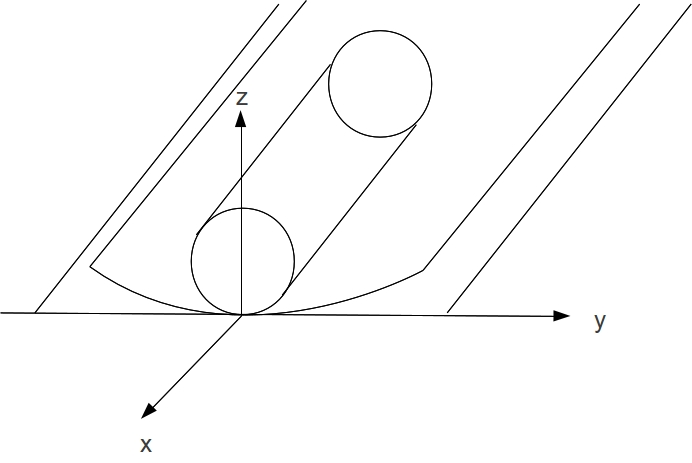
\includegraphics[scale = 0.3]{Bilder/Bsp7.jpg}
  \end{figure}
  \begin{align*}
   (u,v) \in ]-\pi, \pi[ \times \IR \mapsto x(u,v) = \vxyz{h \cdot v}{r \sin u}{r (1-\cos u)} \in \IR^3
  \end{align*}
  ist in die Ebene verbiegbar: Eine stetige Verbiegungsschar ist
  \begin{align*}
   \,^\alpha x(u,v) &= \vxyz{h v}{r \frac1\alpha \sin \alpha u}{r \frac1\alpha (1-\cos \alpha u)} \quad \alpha \in ]0,1] \\
   \,^0 x(u,v) &= \lim_{\alpha \to 0} \,^\alpha x(u,v) = \vxyz{hv}{ru}{0} \quad \text{[Ebenenstück], denn} \\
   \,^\alpha x_1(u,v) &= \vxyz{0}{r\cos \alpha u}{r\sin \alpha u} \\
   \,^\alpha x_2(u,v) &= \vxyz{h}{0}{0} \\
   \Rightarrow \big( \,^\alpha g_{\varrho \sigma}(u,v)\big) &= \begin{pmatrix}
                                                                  r^2 & 0 \\
                                                                  0 & h^2
                                                                 \end{pmatrix}
  \end{align*}
  Die \uline{Tangentialfläche}
  \[
   (s,v) \in I \times \IR \mapsto x(s,v) = c(s) + v T(s) \in \IR^3
  \]
  einer beliebigen wendepunktfreien Kurve \(s \mapsto c(s)\) ist in die Ebene verbiegbar. Es gilt
  \begin{align*}
   \big( \grs(s,v)\big) = \begin{pmatrix}
                           1 + v^2 \kappa^2(s) & 1 \\
                           1 & 1
                          \end{pmatrix}
  \end{align*}
  Die Torsion \(\tau\) der Kurve taucht nicht auf! Nach dem Fundamentalsatz der Kurventheorie kann eine von einem Parameter \(\alpha\) \uline{stetig} abhängende Kurvenschar \(s \mapsto \,^\alpha c(s)\) (\(\alpha \in [0,1]\)) durch Vorgabe von \(s \mapsto \,^\alpha \kappa(s) := \kappa(s)\) und \(s \mapsto \,^\alpha \tau(s) := \alpha \cdot \tau(s)\) konstruiert werden. Die zugehörigen Tangentenflächen bilden eine stetige Verbindungsschar zwischen einem Ebenenstück (\(=\) Tangentenfläche der ebenen Kurve \(\,^0 c\)) und der Ausgangsfläche (\(\alpha = 1\)).
 \end{enumerate}
\end{bsp}

\begin{bemerkung}
 Wir zeigen später, dass die
 \begin{itemize}
  \item \uline{allgemeinen Zylinder}, die 
  \item \uline{allgemeinen Kegel} und 
  \item \uline{Tangentenflächen von Kurven}
 \end{itemize}
 im wesentlichen die einzigen Flächen im \(\IR^3\) sind, die in die Ebene verbiegbar sind. \\
 Name: "`\uline{Torsen}"' \par
 Die Kugel ist \uline{nicht} isometrisch zur Ebene. Deswegen Ärger bei Atlanten (Atlassen).
\end{bemerkung}

\subsection{Hyperflächen im euklidischen $\IR^n$: Ableitungsgleichungen}
Im Folgenden sei \(\uline{p = n-1}\) \qquad 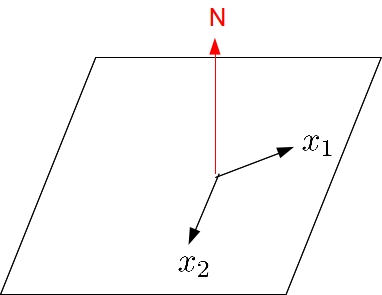
\includegraphics[scale=0.2]{Bilder/Bsp8.jpg}
Offensichtlich gilt

\begin{satz}\label{satz212}
 Ist \(u \in G \mapsto x(u) \in \IR^n\) Parameterdarstellung einer \(\C^1\)-Hyperfläche, so bilden die 
 \begin{itemize}
  \item tangentialen Vektorfelder
  \[
   x_1, \dots, x_{n-1}
  \]
  \item das Normalen(einheits)vektorfeld
  \[
   N := \frac{x_1 \times \dots \times x_{n-1}}{|x_1 \times \dots \times x_{n-1}|}
  \]
 \end{itemize}
 eine \uline{parameterabhängige}, positiv orientierte Begleitbasis\index{Hyperfläche!Begleitbasis} mit den Eigenschaften
 \begin{align*}
  \forall_\varrho \langle x_\varrho, N \rangle &= 0, \quad |N|^2 = 1 \\
  \det (x_1, \dots, x_{n-1}, N) &= \langle x_1 \times \dots \times x_{n-1}, N \rangle = |x_1 \times \dots \times x_{n-1} | = \sqrt{g} = a_{n-1} (x_1, \dots, x_{n-1})
 \end{align*}
 Das Vektorfeld \(N \colon G \to S^{n-1} \subset \IR^n\) ist dabei invariant gegenüber (zulässiger) Parametertransformationen und heißt auch \uline{sphärisches Bild}\index{sphärisches Bild} oder \uline{Gaußabbildung}\index{Gaußabbildung} der Hyperfläche.
\end{satz}

\begin{bemerkung}
 In jedem Punkt \(x(u)\) ist die orthogonale Zerlegung
 \[
  \IR^n = T_u x \stackrel{\perp}{\oplus} \hl N \hr
 \]
 parameterunabhängig.
\end{bemerkung}

\begin{satz}\label{satz213}
 Für die Begleitbasis \((x_1, \dots, x_{n-1}, N)\) einer parametrisierten \(\C^2\)-Hyperfläche gelten (parameter\-\uline{abhängige}) Ableitungsgleichungen der Form 
 \begin{align*}
 &\boxed{\underset{\varrho, \sigma}{\forall}\, x_{\varrho \sigma} = \sum \gamma_{\varrho \;\, \sigma}^{\;\,\mu}\, x_\mu + b_{\varrho \sigma} N} \\
 &\text{[Gaußsche Ableitungsgleichungen]\index{Gaußsche Ableitungsgleichungen]}} \\
 &\boxed{N_\sigma := \partial_\sigma N = - \sum b^\mu_{\;\, \sigma}\, x_\mu [ + 0 \cdot N]} \\
 &\text{[Weingartenschen Ableitungsgleichungen]\index{Weingartenschen Ableitungsgleichungen}}
 \end{align*}
\end{satz}

\begin{beweis}[von Satz \ref{satz213}]
 Klar wegen 
 \[
  |N|^2 = 1 \Rightarrow \langle N_\sigma, N \rangle = 0
 \]
\end{beweis}

\subsubsection*{Berechnung der Koeffizienten}
\begin{enumerate}
 \item[a)] Mit den \uline{Christoffelsymbolen\index{Christoffelsymbole} 1. Art}
 \[
  \gamma_{\varrho \nu \sigma} := \langle x_{\varrho \sigma}, x_\nu \rangle = \sum_\mu \gamma_{\varrho \;\, \sigma}^{\;\,\mu} \, g_{\mu \nu}
 \]
 erhält man die \uline{Christoffelsymbole 2. Art} durch
 \[
  v= \sum_\nu g^{\mu\nu} \, \gamma_{\varrho \nu \sigma}
 \]
 wenn \((g^{\mu\nu})\) die zur \((g_{\varrho \sigma})\) inverse Matrix (mit \(\sum_\nu g^{\mu\nu} \, \grund \nu\sigma = \delta^\mu_{\, \nu}\)) berechnet.
 \item[b)] Es gilt
 \begin{align*}
  b_{\varrho\sigma} &= \langle x_{\varrho\sigma}, N \rangle = -\langle x_{\varrho}, N_\sigma \rangle = + \sum_\mu b^\mu_{\;\,\sigma} \, g_{\mu \varrho} \\
  \Rightarrow b^\mu_{\;\,\sigma} &= \sum_{\varrho} g^{\mu\varrho} \, b_{\varrho\sigma}
 \end{align*}
\end{enumerate}

\begin{bemerkung}\(\)
\begin{enumerate}
 \item Mit den Matrizen \((g_{\varrho\sigma})\) und ihrer Inversen \((g^{\varrho \sigma})\) lassen sich im Tensorkalkül Indizes "`herauf- und herunterziehen"'.
 \item \((\gamma_{\varrho\nu\sigma}),\, (\gamma_{\varrho \;\, \sigma}^{\;\,\mu}),\, (v_{\varrho \sigma})\) sind in dem Indexpaar \((\varrho, \sigma)\) \uline{symmetrisch}.
 \begin{align*}
 (b^\mu_{\;\,\sigma}) = (g^{\mu\nu}) \cdot (b_{\varrho \sigma})
 \end{align*}
 braucht \uline{nicht} symmetrisch sein, obwohl Produkt symmetrischer Matrizen!
 \item Bei \(n = 3\) denke man an \(N = \frac1{\sqrt{g}} x_1 \times x_2\)
 \begin{align*}
 (g^{\varrho \sigma}) &= \frac1g \begin{pmatrix}
                                 g_{22} & -g_{12}\\
                                 -g_{21} & g_{11}
                                \end{pmatrix} \\
 (b^\mu_{\;\,\sigma}) &= \begin{pmatrix}
                        b^1_{\;\,1} & b^1_{\;\,2} \\
                        b^2_{\;\,1} & b^2_{\;\,2}
                       \end{pmatrix}         
 \end{align*}
\end{enumerate}

\end{bemerkung}

\subsubsection*{Fragen}
\begin{enumerate}
 \item Welche geometrische und algebraische Bedeutung haben die Koeffizienten \(\gamma_{\varrho \;\, \sigma}^{\;\,\mu}, \, b_{\varrho\sigma},\, b^\mu_{\;\,\sigma}\)?
 \item Wie ändern sie sich bei Parametertransformationen? (z.T. kompliziert, Berechnung soll vermieden werden)
 \item Wie kann man die Ableitungsgleichungen parameterunabhängig formulieren?
\end{enumerate}

\subsubsection*{Idee (zu 3.)}
Statt die parameterabhängigen Vektorfelder \(x_1, \dots, x_{n-1}, N\) in Richtung von Parameterlinien (nach \(u^\sigma\)) zu differenzieren, Ableiten eines \uline{beliebigen} (tangentialen oder normalen) Vektorfeldes \(u \mapsto Z(u)\) in Richtung eines \uline{beliebigen} Vektors \(Y \in T_u x\). Diese \uline{Richtungsableitung}\index{Richtungsableitung}
\begin{align*}
 \boxed{\dd_Y Z = \sum (\partial_\sigma Z) Y^\sigma}
\end{align*}
(mit \(Y = \sum Y^\sigma x_\sigma\)) [vergleiche im \(\IR^n\): \(d_Y f = \langle \grad f, Y \rangle = \sum \partial_\varrho f \cdot Y^\varrho\)]\par
ist \uline{parameterunabhängig}, denn aus \(x = \widetilde x \circ \Phi, \, Z = \widetilde Z \circ \Phi, \, Y = \widetilde Y \circ \Phi\) folgt	
\begin{align*}
 &\dd_Y Z(u) = \sum_\sigma \partial_\sigma \left( \widetilde Z \big( \Phi(u)\big)\right) Y^\sigma(u) = \sum_{\mu,\sigma} \left( \partial_\mu \widetilde Z\right) \big(\Phi(u)\big) \underbrace{\frac{\partial \widetilde u^\mu}{\partial u^\sigma} Y^\sigma(u)}_{\widetilde Y^\mu \big(\Phi(u)\big)} = \uline{\dd_{\widetilde Y} \widetilde Z} \big(\Phi(u)\big) \\
 &\left(\text{weil } x_\varrho = \sum \widetilde u_\varrho^\sigma \,\widetilde x_\sigma \Leftrightarrow \widetilde Y^\sigma = \sum \widetilde u_\varrho^\sigma \, Y^\varrho\right)
\end{align*}

\subsubsection{Eigenschaften des linearen Differentialoperators}
\[
 d \colon (Z,Y) \mapsto \dd_Y Z
\]
\begin{enumerate}
 \item[1a)] Additivität in \(Z\):
 \[
  \dd_Y (Z_1 + Z_2) = \dd_Y Z_1 + \dd_Y Z_2
 \]
 \item[1b)] Derivativität in \(Z\):
 \[
  \dd_Y(f \cdot Z) = (\dd_Y f)Z + f \dd_Y Z
 \]
 \item[2)] Linearität in \(Y\):
 \[
  \dd_{f_1 Y_1, f_2 Y_2} Z = f_1 \dd_{Y_1} Z + f_2 \dd_{Y_2} Z
 \]
\end{enumerate}
Da auch die Zerlegung von \(u \mapsto \dd_Y Z(u)\) in Tangential- und Normalanteil parameterunabhängig ist, erhält man folgende invariante Darstellung: \par
Für \(Z = X\) selbst tangential gilt
\begin{align*}
 \dd_Y X &= \sum \partial_{\sigma} \left( \sum X^{\cancelto{\mu}{\varrho}} x_{\cancelto{\mu}{\varrho}}\right)Y^\sigma = \sum \left( \partial_\sigma X^\varrho \right) Y^\sigma x_\varrho + \sum X^\varrho x_{\varrho \sigma} X^\sigma \\
 &=\underbrace{\sum \left[ \left( \partial_\sigma X^\mu + X^\varrho \christ \gamma \varrho \mu \sigma \right) Y^\sigma \right] x_\mu}_{\dd_Y X |_\perp} + \underbrace{\left[ \sum b_{\varrho \sigma} X^\varrho Y^\sigma \right]}_{\langle \dd_Y X, N\rangle = \langle- X, \dd_Y N \rangle (\text{(Bilinearform)})} N \\
 &=: \nabla_Y X + \Rom 2 (X,Y) N
\end{align*}
und für \(Z = N\):
\begin{align*}
 \dd_Y N = \sum \left( \partial_\sigma N\right) Y^\sigma = - \sum \wein \mu \sigma Y^\sigma x_\mu = -A(Y) \quad \text{(lineare Abbildung)}
\end{align*}

\uline{Ergebnis}:

\begin{satz}\label{satz214}
 Auf einer \(\C^2\)-Hyperfläche in einer Parametrisierung \(u \mapsto x(u) \) erfüllen tangentiale \(\C^1\)-Vektorfelder \(u \mapsto X(u)\) un das Normalenvektorfels \(u \mapsto N(u)\) die (parameterunabhängigen) \uline{Ableitungsgleichun}\-\uline{gen}
\begin{align*}
 \dd_Y X &= \nabla_Y X + \Rom 2 (X,Y) N & \text{(Gaußsche Ableitungsgleichung)} \\
 \dd_Y N &= -A (Y) & \text{(Weingartensche Ableitungsgleichung)}
\end{align*}
in Richtung tangentialer Vektorfelder \(u \mapsto Y(u)\). \par
Dabei gilt:
\begin{enumerate}
 \item[a)] Durch \((X,Y) \mapsto \nabla_Y X = \dd_Y X |_T\) wird ein linearer Differentialoperator definiert, der je zwei tangentialen Vektorfeldern \(X,Y\) wieder ein tangentiales Vektorfeld \(\nabla_Y X\) zuordnet, genannt \uline{kovariante Ableitung}\index{kovariante Ableitung} von \(X\) in Richtung \(Y\). \\
 (Andere Bezeichnung: Durch \(\nabla\) wird ein \uline{linearer Zusammenhang}\index{linearer Zusammenhang} (linear connection) definiert)
 \item[b)] Durch \((X,Y) \mapsto \Rom 2(X,Y) = \langle \dd_Y X, N\rangle = -\langle X, \dd_Y N \rangle = -\Rom 1 (X, \dd_YN)\) wird ein Feld symmetrischer \uline{Bilinearformen} 
 \[
  \Rom 2 u \colon T_u x \times T_u x \to \IR, \, (X,Y) \mapsto \Rom 2_u (X,Y)
 \]
 definiert, genannt \uline{2. Grundform}\index{2. Grundform} (2. Fundamentalform) der Hyperfläche
 \item[c)] Durch \(Y \mapsto A(Y) := -\dd_Y N\) wird ein Feld \uline{linearer Abbildungen} \(A_u \colon T_u x \to T_u x\) definiert, genannt \uline{Weingarten-Endomorphismus}\index{Weingarten-Endomorphismus} (shape operator) der Hyperfläche.
\end{enumerate}

\end{satz}

\begin{folgerung}[Interpretation von \(\christ \varrho \mu \sigma\), \(b_{\varrho \sigma}\), \(\wein \mu \sigma\)]
 Bezüglich einer festen Parametrisierung \(u \mapsto x(u)\) einer \(\C^2\)-Hyperfläche hat man die Basisdarstellung (setze \(X = X_\varrho, Y = X_\sigma\))
 \begin{align*}
  \nabla_\sigma X_\varrho &:= \nabla_{x_\sigma} x_\varrho = \sum \christ \varrho \mu \sigma x_\mu \\
  \Rom 2 (x_\varrho, x_\sigma) &= b_{\varrho \sigma} \\
  A(x_\sigma) &= + \sum \wein \mu \sigma x_\mu
 \end{align*}
Die Christoffelsymbole \(\christ \varrho \mu \sigma\) sind also die \uline{Darstellungskoeffizienten} der kovarianten Ableitung \(\nabla\) (auch als \uline{Zusammenhangskoeffizienten} bezeichnet), \\
die symmetrische Matrix \((b_{\varrho \sigma})\) ist die \uline{Darstellungsmatrix} der 2. Grundform \(\Rom 2\) und \\
die (im Allgemeinen nicht symmetrische) Matrix \((\wein \mu \sigma )\) die \uline{Darstellungsmatrix} des Weingarten-Endomorphismus \(A\), jeweils bezüglich der Basisfelder \(u \mapsto \big(x_1, \dots, x_{n-1}\big) (u)\) \par
Umgekehrt gilt (bezüglich jeder Parametrisierung):
\begin{align*}
 \nabla_Y X &= \sum \left[ \partial_\sigma X^\mu + X^\varrho \christ \varrho \mu \sigma Y^\sigma \right] x_\mu \\
 \Rom 2 (X,Y) &= \sum b_{\varrho \sigma} X^\varrho Y^\sigma \\
 A(Y) &= \sum \wein \mu \sigma Y^\sigma x_\mu
\end{align*}
Früher übliche Bezeichnung für \(p = 2, n = 3\)
\[
 (b_{\varrho \sigma} = \begin{pmatrix}
                        L & M \\
                        M & N
                       \end{pmatrix} = 
                       \begin{pmatrix}
                        e & f \\
                        f & g
                       \end{pmatrix}
\]
\end{folgerung}

(Für Profis: \(\nabla\) ist der von der Metrik \(\Rom 1\) induzierte Levi-Civita-Zusammenhang.)

\subsubsection{Grundlegende Eigenschaften von \(\nabla, \, \Rom 2, \, A\)}
\begin{enumerate}
 \item[(1)] Die kovariante Ableitung \(\nabla\) (bezüglich ihrer Koeffizienten \(\christ \varrho \mu \sigma\)) ist eine \uline{innergeometrische Größe}
\end{enumerate}

\begin{satz}\label{satz215}
 ie Christoffelsymbole 1. und 2. Art einer \(\C^2\)-(Hyper)Fläche lassen sich allein aus den Komponenten \(g_{\varrho \sigma}\) der 1. Grundform bestimmen. Und zwar gilt
 \begin{align*}
  \gamma_{\varrho \mu \sigma} = \frac12 \left( \partial_\varrho g_{\nu \sigma} - \partial_\nu g_{\varrho \sigma} + \partial_\sigma g_{\varrho \nu}\right)
 \end{align*}
\end{satz}

\begin{beweis}[von Satz \ref{satz215}]
 Aus 
 \begin{align*}
  \partial_\varrho g_{\nu \sigma} &= \partial_\varrho \langle x_\nu, x_\sigma \rangle + \langle x_\nu x_{\sigma \varrho} \rangle &= \gamma_{\nu\sigma\varrho} + \gamma_{\sigma \nu \varrho} \\
  \partial_\nu g_{\varrho \nu} &= \dots &= \gamma_{\varrho \sigma \nu} + \gamma_{\sigma \varrho \nu} \\
  \partial_\sigma g_{\varrho \nu} &= \dots &= \gamma_{\nu \varrho \sigma} + \gamma_{\varrho \nu \sigma}
 \end{align*}
 und der Symmetrie \(\gamma_{\varrho \nu \sigma} = \gamma_{\sigma \nu \varrho}\) die Behauptung.
\end{beweis}

\begin{enumerate}
 \item[(2)] Die Weingarten-Matrizen \((\wein \mu \sigma )\) bezüglich verschiedener Parametrisierungen sind (als Darstellungsmatrizen desselben Endomorphismus \(A\)) \uline{ähnlich} zueinander. \\
 (Parameterunabhängige) \uline{Invarianten} sind also ihre elementarsymmetrischen Funktionen (\(=\) Koeffizienten des charakteristischen Polynoms), insbesondere Spur und Determinante.
\end{enumerate}

\begin{definition}
 Bei einer \(\C^2\)-Hyperfläche im \(\IR^n\) heißt 
 \[
  H:= \frac{1}{n-1} \tr A = \frac{1}{n-1} \sum \wein \varrho \varrho
 \]
 die \uline{mittlere Krümmung}\index{mittlere Krümmung} und
 \[
  \kappa := \det A = \det (\wein \mu \sigma)
 \]
 die \uline{Gaußsche Krümmung}\index{Gaußsche Krümmung}
\end{definition}

\begin{bemerkung}
 Aus \((\wein \mu \sigma ) = (g^{\stackrel{\alpha}{\varrho}\stackrel{\beta}{\sigma}}) \cdot (b_{\varrho \sigma})\) folgt 
 \[
  \kappa = \frac{b}{g} = \frac{\det (b_{\varrho \sigma})}{\det (g_{\varrho \sigma})}
 \]
\end{bemerkung}

\begin{enumerate}
 \item[(3)] Der Weingarten-Endomorphismus \(A\) ist \uline{selbstadjungiert}. Für tangentiale Vektorfelder \(X,Y\) gilt \(\langle X, Y\rangle = 0\), also 
 \begin{align*}
  \dd_Y \left[ \langle X,N \rangle \right] &= \langle \dd_Y X, N \rangle + \langle X, \dd_Y N \rangle = \Rom 2 (X,Y) - \langle X;A(Y) \rangle \\
  &=\Rom 2 (X,Y) - \Rom 1\big(Y, A(Y)\big) = 0 \\
  (\text{in Koordinaten: } &= b_{\varrho \sigma} - \sum g_{\varrho \mu} \wein \mu \sigma )
  \end{align*}
  Die Symmetrie von \(\Rom 2\) liefert
\end{enumerate}

\begin{satz}\label{satz216}
 Die Weingartenabbildung \(A_u \colon T_u x \to T_u x\) ist in jedem Punkt \(x(u)\) einer Hyperfläche \uline{selbstadjungiert} bezüglich des Skalarprodukts \(\Rom 1_u\) auf \(T_u x\), d.h. es gilt überall
 \[
  \Rom 1 \big(X, A(Y)\big) = \Rom 1 \big(A(X), Y\big)
 \]
 Sie besitzt demnach nur \uline{reelle Eigenwerte} und eine \uline{Orthonormalbasis aus Eigenvektoren}.
\end{satz}

\begin{bemerkung}
 Obwohl \(A\) selbstadjungiert ist, sind die Darstellungsmatritzen \((\wein \mu \sigma)\) in \(A\) nicht \uline{symmetrisch}.
\end{bemerkung}

\subsubsection{Bezeichnungen}
Eigenwert von \(A_u\):
\[
 \kappa_1(u), \dots, \kappa_{n-1}(u) \quad \text{\uline{Hauptkrümmungen}}
\]
Orthonormierte Eigenvektoren dazu:
\[
 Y_1(u), \dots, Y_{n-1}(u) \quad \text{\uline{Hauptkrümmungsrichtungen}}
\]

\subsubsection{Zusammenfassung Krümmungsinvarianten aus den Weingartenabbildungen \(Y \mapsto A(Y) = -\dd_Y N\)}
\begin{align*}
 &H = \frac{1}{n-1} \tr A & \text{Mittlere Krümmung} \\
 &\kappa = \det A & \text{Gaußsche Krümmung} \\
 &\kappa_1, \dots, \kappa_{n-1} & \text{Hauptkümmungen = Eigenwerte von }A \\
 &Y_1, \dots, Y_{n-1} & \text{Hauptkrümmung = Eigenvektoren von }A \text{(Orthonormalbasis!)}
\end{align*}

\begin{folgerung}
 Wegen \(A(Y_\varrho) = \kappa_\varrho Y_\varrho (\varrho = 1, \dots, n-1)\) gilt
 \begin{align*}
  &H = \frac{1}{n-1} (\kappa_1 + \dots + \kappa_{n-1} & \text{(deswegen \uline{mittlere} Krümmung)} \\
  & \kappa = \kappa_1 \cdot \dots \cdot \kappa_{n-1}
 \end{align*}
Zur geometrischen Bedeutung: siehe Kapitel 2.3
\end{folgerung}

\subsubsection{Vorgriff ($n=3$)}
Flächen mit \(H \equiv 0\) heißen \uline{Minimalflächen} \\
Flächen mit \(\kappa \equiv 0\) heißen \uline{Torsen} (\(=\) ``flache Flächen'') \\
Formelsammlung: siehe Homepage J. König.
\subsubsection{Ergänzung}
Oft sind tangentiale Vektorfelder nur längs einer Flächenkurve \(t \mapsto c(t) = x\big(u(t)\big)\) in der Form 
\[
 t \mapsto X(t) = \sum X^\varrho(t)x_{\varrho}\big(u(t)\big)
\]
gegeben.
\begin{bsp}
  \mat{X(t) := \dot c(t) = \sum \dot u^\varrho(t)x_\varrho \big(u(t)\big)}
  \uline{kovariante Ableitung}:
  \begin{align*}
   \frac{\nabla X}{\dd t} &:= \left.\frac{\dd X}{\dd t} \right|_T = \sum \left[\dot X^{\cancelto{\mu}{\varrho}} x_{\cancelto{\mu}\varrho} \;\,(u) + X^\varrho x_{\varrho \sigma} (u)|_\perp \cdot \dot u^\sigma\right] \\
   &= \uline{\sum \left( \dot X^\mu + X^\varrho \christ \varrho \mu \sigma (u) \dot u^\sigma \right) x_\mu(u)}
  \end{align*}
\end{bsp}

\section{Zur inneren Geometrie der Flächen im $\IR^3$}
Im Folgenden sei \(p = 2, n = 3\); das meiste gilt für beliebige \(p\). \par
In der euklidischen Ebene sind wohldefinierte:
\begin{itemize}
 \item die \uline{Parallelverschiebung}\index{Parallelverschiebung} eines Vektors \(X_0\) längs einer Kurve \(t \mapsto c(t)\). Sie liefern ein \uline{Parallelfeld}\index{Parallelfeld} \(t \mapsto X(t)\) mit \(\frac{\dd X}{\dd t} = 0\), d.h. \(X = X_0 = \const.\)
 \item \uline{gerade Linien}, etwa mit der Kennzeichnung \(\frac{\dd T}{\dd t} \equiv 0\), d.h. \(T = \const.\)
\end{itemize}
Übertragung der Begriffe auf ``krumme'' Flächen durch Rückprojektion der Ableitungsvektoren \(\frac{\dd X}{\dd t}\) bzw. \(\frac{\dd T}{\dd t}\) in die Tangentialebene, d.h. Benutzung der (innergeometrischen) kovarianten Ableitung \(\frac{\nabla X}{\dd t}\) bzw. \(\frac{\nabla T}{\dd t}\). \\
(Vektorfelder sind nur so parallel bzw. Kurven nur so gerade, wie die Fläche es zulässt.

\subsection{Geodätische Parallelverschiebung}
\Rechts
\begin{definition}
 Ein tangentiales \(\C^1\)-Vektorfeld \(t \mapsto X(t) = \sum X^\varrho (t) x_\varrho \big(u(t)\big)\) längs einer \(\C^1\)-Flächenkurve \(t \mapsto c(t) = x\big(u(t)\big)\) heißt \uline{geodätisch parallel}\index{geodätische Parallelität}, wenn gilt
 \begin{align*}
  &\frac{\nabla X}{\dd t} = \left.\frac{\dd X}{\dd t}\right|_T \equiv 0, \text{ also} \\
  &\dot X^\mu + \sum X^\varrho \christ \varrho \mu \sigma (u) \dot u^\sigma = 0 \quad (\mu = 1,2) \tag{\(\ast\)}
 \end{align*}
(d.h. der innergeometrisch nur sichtbare Anteil der Ableitung verschwindet) \par
\((\ast)\) ist ein \uline{lineares} Differentialgleichungssystem 1. Ordnung für die Komponentenfunktionen \(t \mapsto X^\mu (t)\, (\mu = 1,2)\), das unter Anfangsbedingungen \(X^\mu(t_0) = X_0^\mu\, (\mu = 1,2)\) eindeutig gelöst werden kann.5
\end{definition}

\begin{folgerung}
 Ein Tangentialvektor auf einer \(\C^2\)-Fläche lässt sich längs jeder \(\C^1\)-Flächenkurve eindeutig geodätisch parallelverschieben. Bei Parallelverschiebung bleiben metrische Größen erhalten:
\end{folgerung}

\begin{satz}\label{satz221}
 Sind \(t \mapsto X(t) = \sum X^\varrho (t) x_\varrho\big(u(t)\big), \, Y(t) = \sum X^\sigma(t) x_\sigma \big(u(t)\big)\) geodätisch parallele \(\C^1\)-Vektorfelder längs derselben \(\C^1\)-Flächenkurve \(t \mapsto c(t) = x\big(u(t)\big)\), so gilt
 \begin{align*}
  t \mapsto Rom 1_{u(t)}\big(X(t), Y(t)\big) = \sum g_{\varrho \sigma} \big(u(t)\big) X^\varrho(t) Y^\sigma(t) = \const.
 \end{align*}
d.h. Längen, Winkel, Flächeninhalt bleiben erhalten.
\end{satz}
Der Satz kann ``innergeometrisch'' bewiesen werden. \\
kürzer: ``außergeometrisch''

\begin{beweis}[von Satz \ref{satz221}]
 \begin{align*}
  \frac{\dd}{\dd t} \left( \Rom 1_{u(t)} \big( X(t), Y(t) \big)\right) &= \frac{\dd}{\dd t} \langle X(t), Y(t)\rangle = \left\langle \frac{\dd X}{\dd t}(t), Y(t) \right\rangle + \left\langle X(t), \frac{\dd Y}{\dd t}(t)\right\rangle \\
  &= \left\langle \underbrace{\frac{\nabla X}{\dd t} (t)}_{=0}, Y(t) \right\rangle + \left\langle X(t), \underbrace{\frac{\nabla Y}{\dd t}(t)}_{=0} \right\rangle =0
 \end{align*}

\end{beweis}

\begin{bsp}[für geodätische Parallelfelder (ohne Rechnung!)]
 Benutzte Eigenschaften:
 \begin{enumerate}
  \item In der \uline{Ebene} gilt ``parallel'' = ``geodätisch parallel''
  \item \uline{Berühren} sich zwei Flächen längs einer Flächenkurve, so ist der geodätische Parallelismus bezüglich dieser Kurven für beide Flächen derselbe (denn es wird in die gleiche Tangentialebene projeziert)
 \end{enumerate}
\uline{Kreiszylinder} 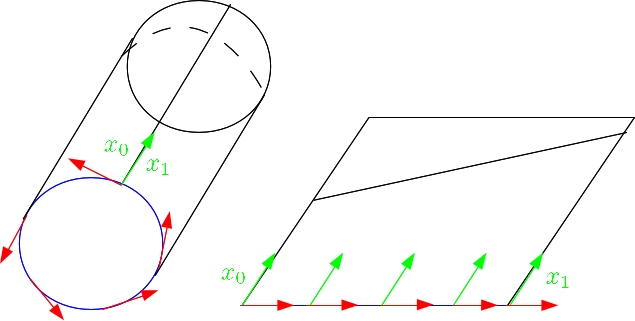
\includegraphics[scale=0.2]{Bilder/Bsp9} \par
\uline{Kreisgekel} 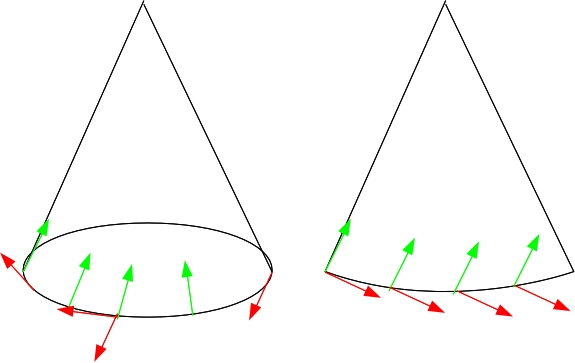
\includegraphics[scale=0.2]{Bilder/Bsp10} \par
\uline{Großkreis} 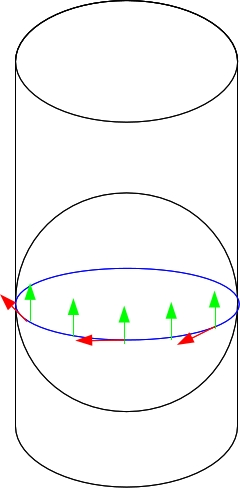
\includegraphics[scale=0.2]{Bilder/Bsp11} 
grüne Pfeile: Parallelfeld längs Großkreis \\
roter Pfeil: Tangentenvektoren bilden Parallelfeld (berühren Zylinder) \par
\uline{Kleinkreis} 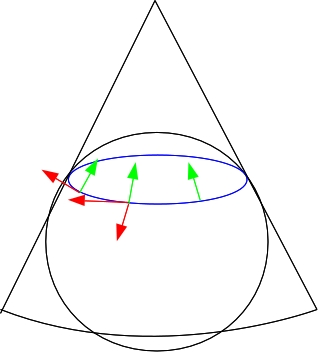
\includegraphics[scale=0.2]{Bilder/Bsp12}
grüner Pfeil: Parallelfeld längs Kleinkreis \\
roter Pfeil: Tangentenvektoren bilden \uline{kein} Parallelfeld \par
Geodätische Parallelverschiebung ist im Allgemeinen nicht wegunabhängig. 
\begin{figure}[ht]
 \centering
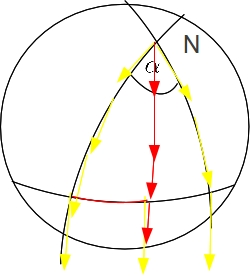
\includegraphics[scale=0.3]{Bilder/Bsp13}
\end{figure}
\end{bsp}
